%% Preamble
% Document type, packages imported, theme and color:
\documentclass{beamer}
\usepackage{amsmath,geometry,graphicx}
\usetheme{Madrid}
\usepackage{multicol}

% Title page
\title{Light reflections}

\date{July 25, 2018}
\author{
Michael Byrne, 
Fatoumata Sanogo,
Pai Song,
Kevin Tsai,
Hang Yang, and
Li Zhu\\
\medskip
Problem Presenter:  John Peach (MIT Lincoln Lab)\\
Faculty Mentor: Alen Alexanderian (NCSU)
}
\titlegraphic{}
\institute[Abbreviation]{SAMSI-IMSM}

%% Presentation
\begin{document}

\begin{frame}
\titlepage
\end{frame}

\begin{frame}[t] 
\frametitle{Motivation} 
\begin{itemize} 
\item Satellite tracking 
\item Prediction of reflective response 
\item Guide model calibration 
\vspace{2mm}
\end{itemize} 
\centerline{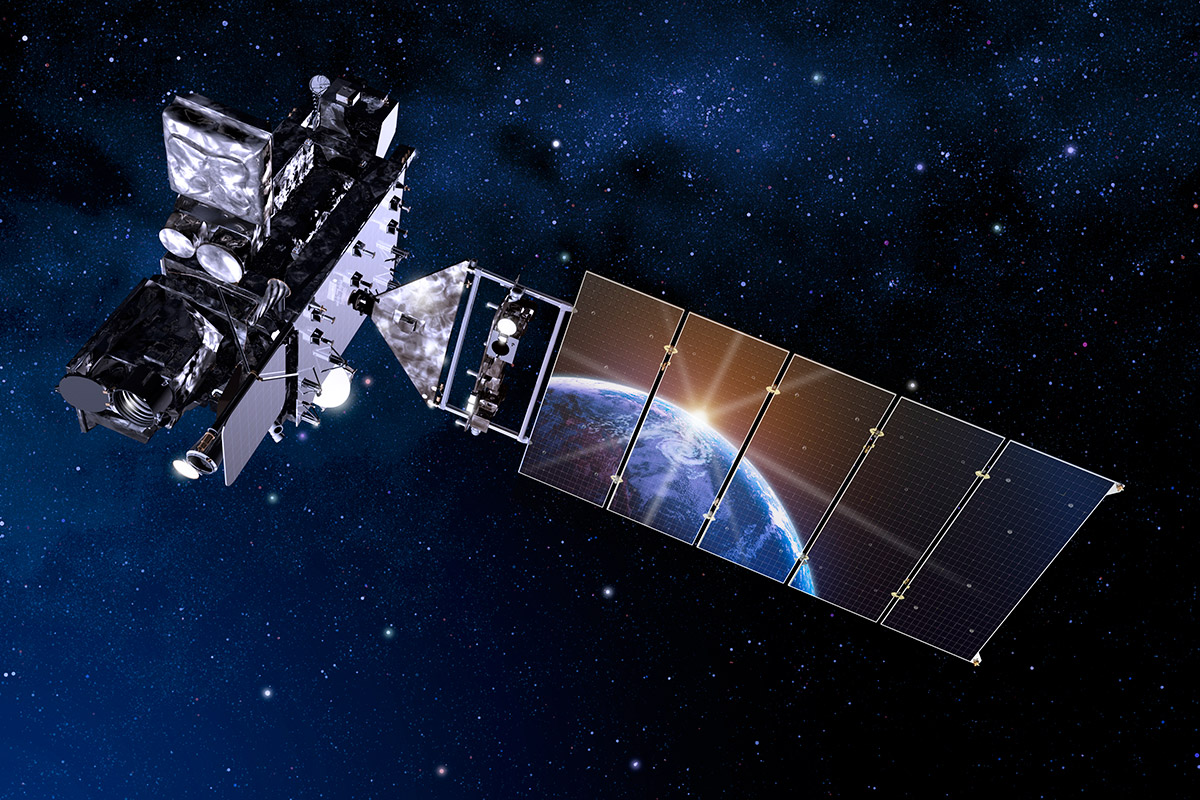
\includegraphics[width = 0.5\linewidth]{./figs/Satellite.jpg}} 
\end{frame} 
 
\begin{frame} 
\frametitle{Goals} 

\begin{columns}
\begin{column}{0.5\textwidth}
\begin{itemize} 
\item Build complex objects using various methods (OpenSCAD, R-functions) 
\item Develop a continuous approach to optical cross section (OCS) computation 
\item Find a solution to the multipath problem 
\end{itemize} 
\end{column}
\begin{column}{0.5\textwidth}
\centerline{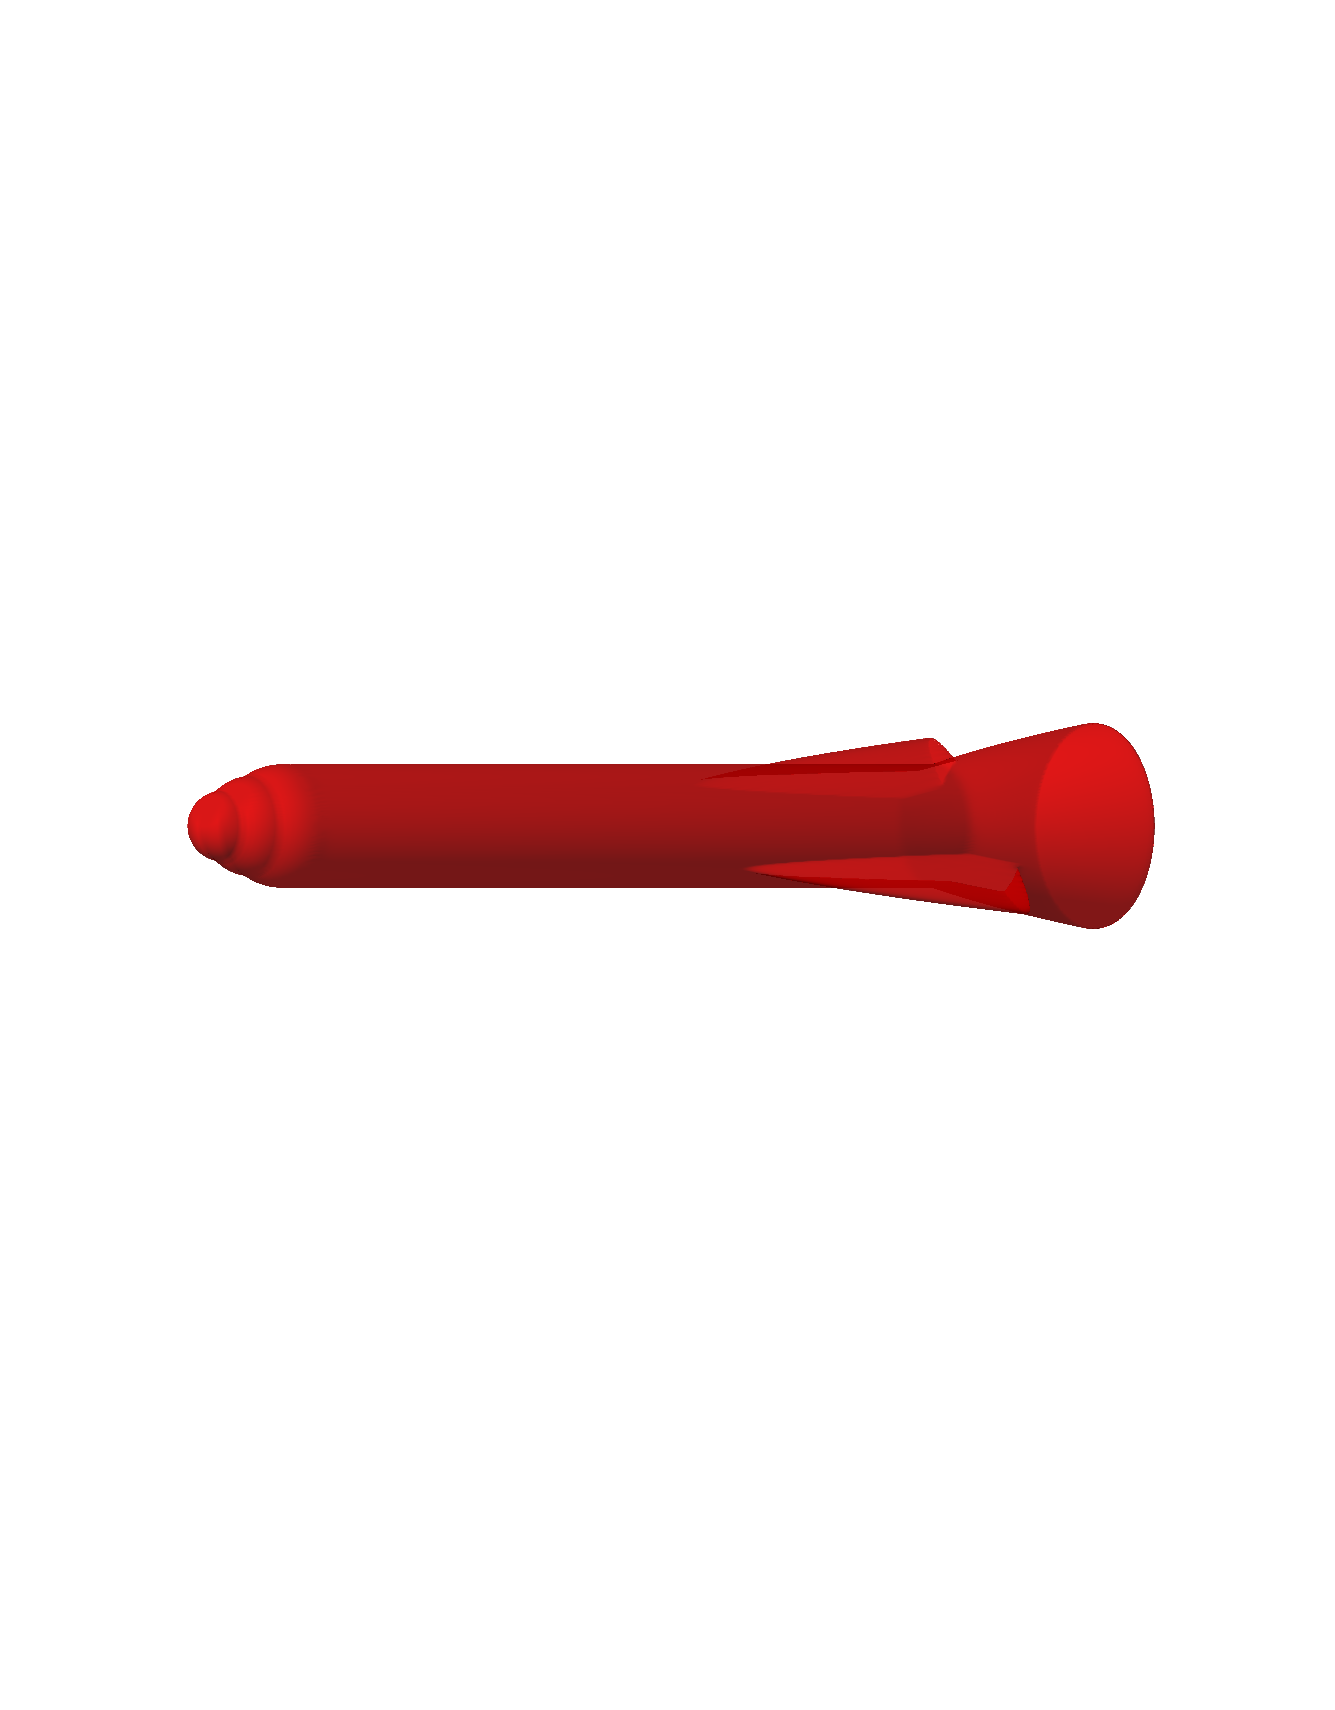
\includegraphics[width = 0.6\linewidth]{rocket.pdf}}\\ 
\vspace{5mm}
\centerline{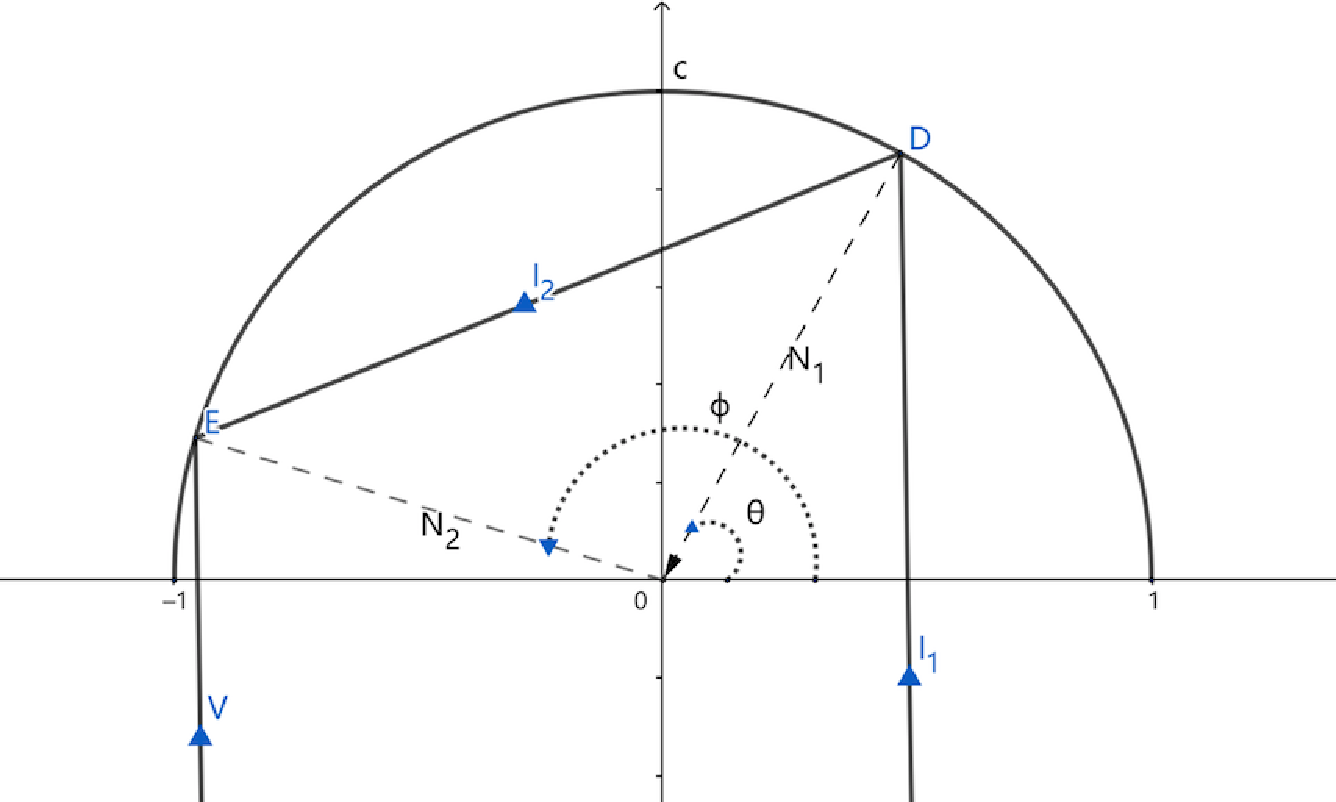
\includegraphics[width = 0.6\linewidth]{./figs/multipath.pdf}}
\end{column}
\end{columns}

\end{frame} 

\begin{frame}
\frametitle{OpenSCAD} 
\centerline{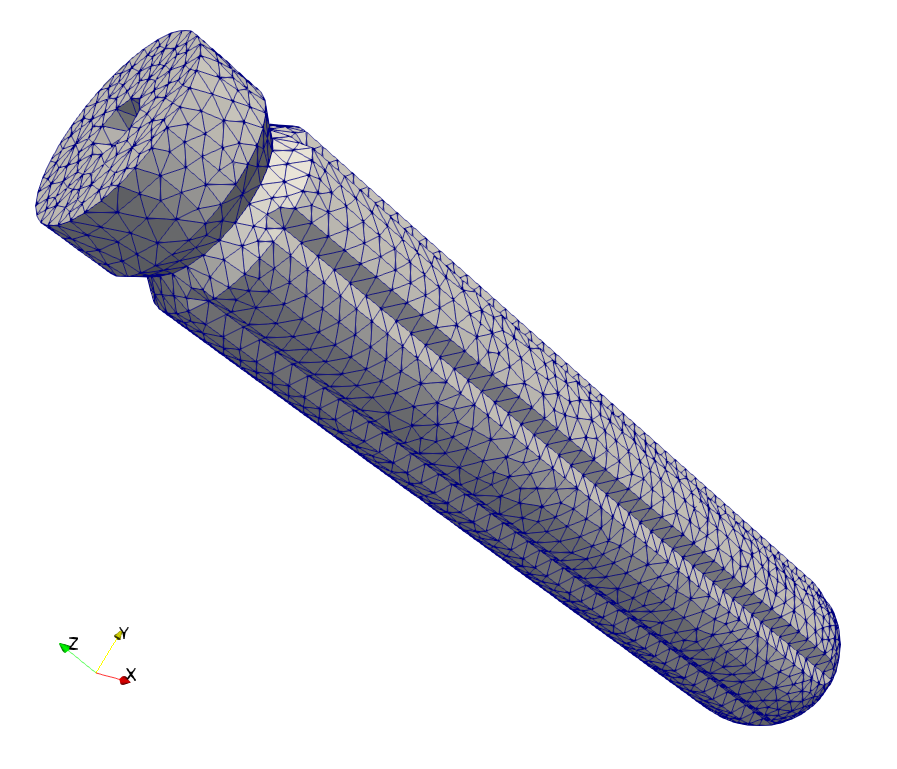
\includegraphics[scale = 0.3]{./figs/sdh_mesh}} 
\end{frame}

\begin{frame}[t] 
\frametitle{Rvachev functions (1963)} 
\begin{itemize} 
\item Commonly referred to as R-functions 
\item Inputs are implicit functions
\item Boolean algebra to construct composite shapes from simple ones 
\[
    \begin{aligned}
    f \cap g &= f + g + \sqrt{f^2 + g^2}       \\ 
    g \cup g &= f + g - \sqrt{f^2 + g^2}       \\
    f \setminus g &= f - g - \sqrt{f^2 + g^2}  \\
    \end{aligned}
\]
\end{itemize} 
\end{frame}
\begin{frame}[t] 
\frametitle{R-functions --- example} 
Union of two spheres:
\[
   \begin{aligned}
   f&: x^2+y^2+z^2 - 1 &= 0 \\
   g&: (x-1)^2+y^2+z^2 - 1 &= 0 \\
   \end{aligned}
\]


\begin{center}
{\tiny
\centerline{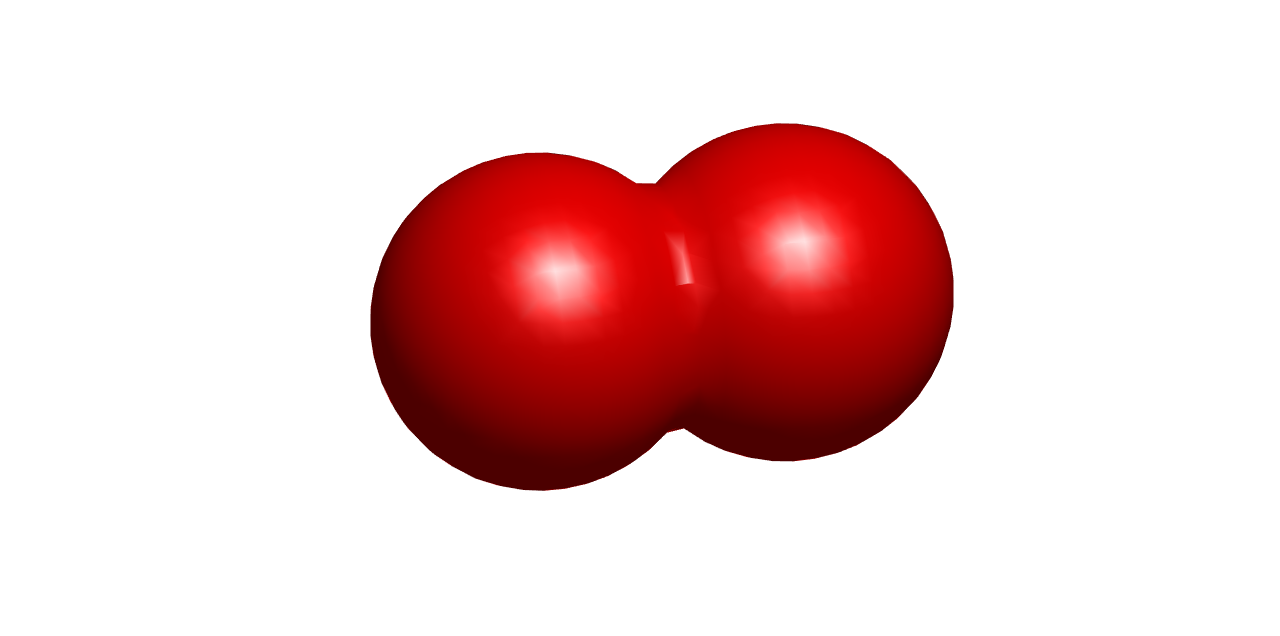
\includegraphics[width = 0.75\linewidth]{./figs/TwoSpheres}} 
\vspace{-3mm}
$
f \cup g: {\left(x-\frac{3}{2}\right)}^2-\sqrt{{\left(x^2+y^2+z^2-1\right)}^2+{\left({\left(x-\frac{3}{2}\right)}^2+y^2+z^2-1\right)}^2}+x^2+2\,y^2+2\,z^2-2 = 0$ 
}
\end{center}
\end{frame} 

\begin{frame}
\frametitle{R-functions more examples} 
\centerline{\begin{tabular}{cc}
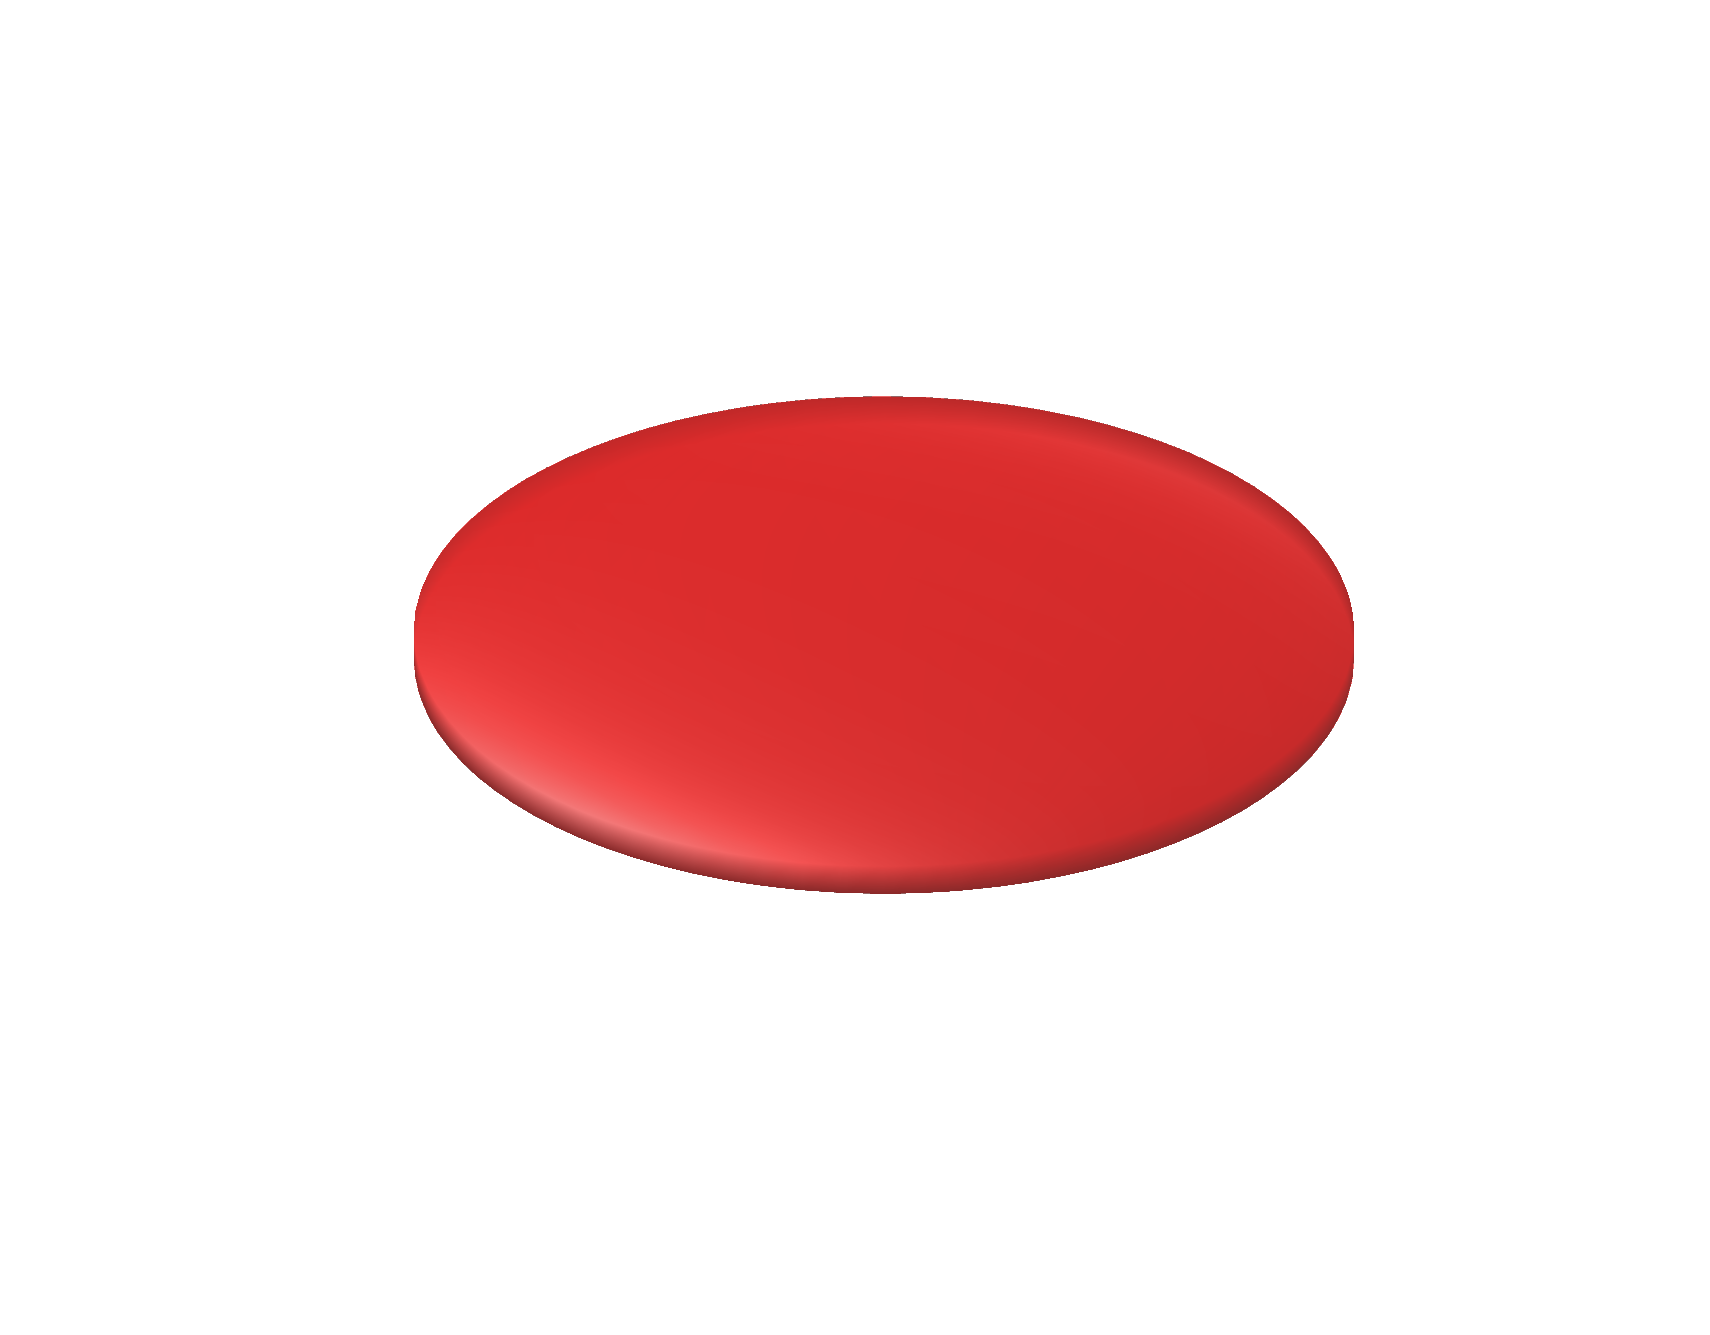
\includegraphics[width=.32\textwidth]{./figs/shape1.pdf} &
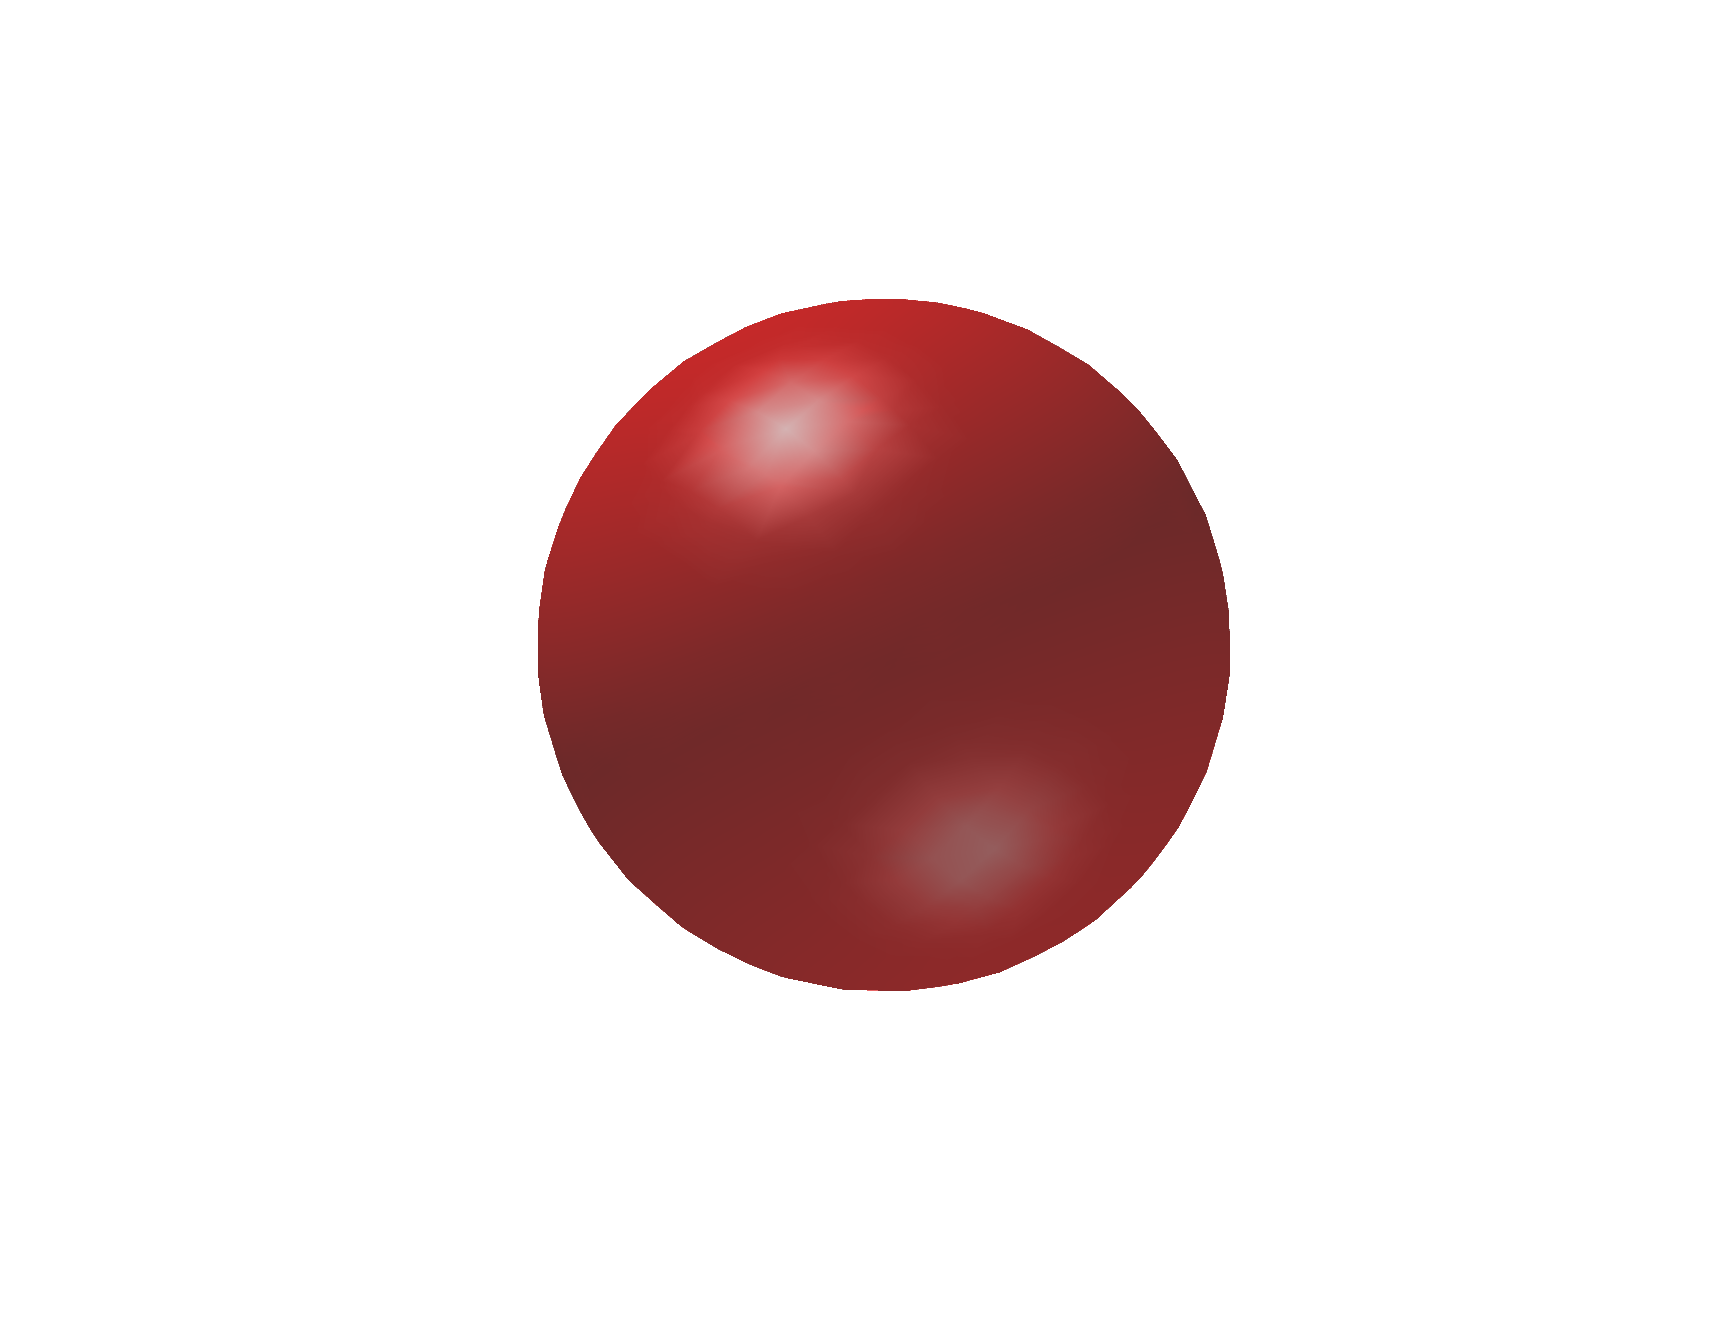
\includegraphics[width=.32\textwidth]{./figs/shape2.pdf}  
\\
$f$ & $g$
\end{tabular}}
\begin{tabular}{ccc}
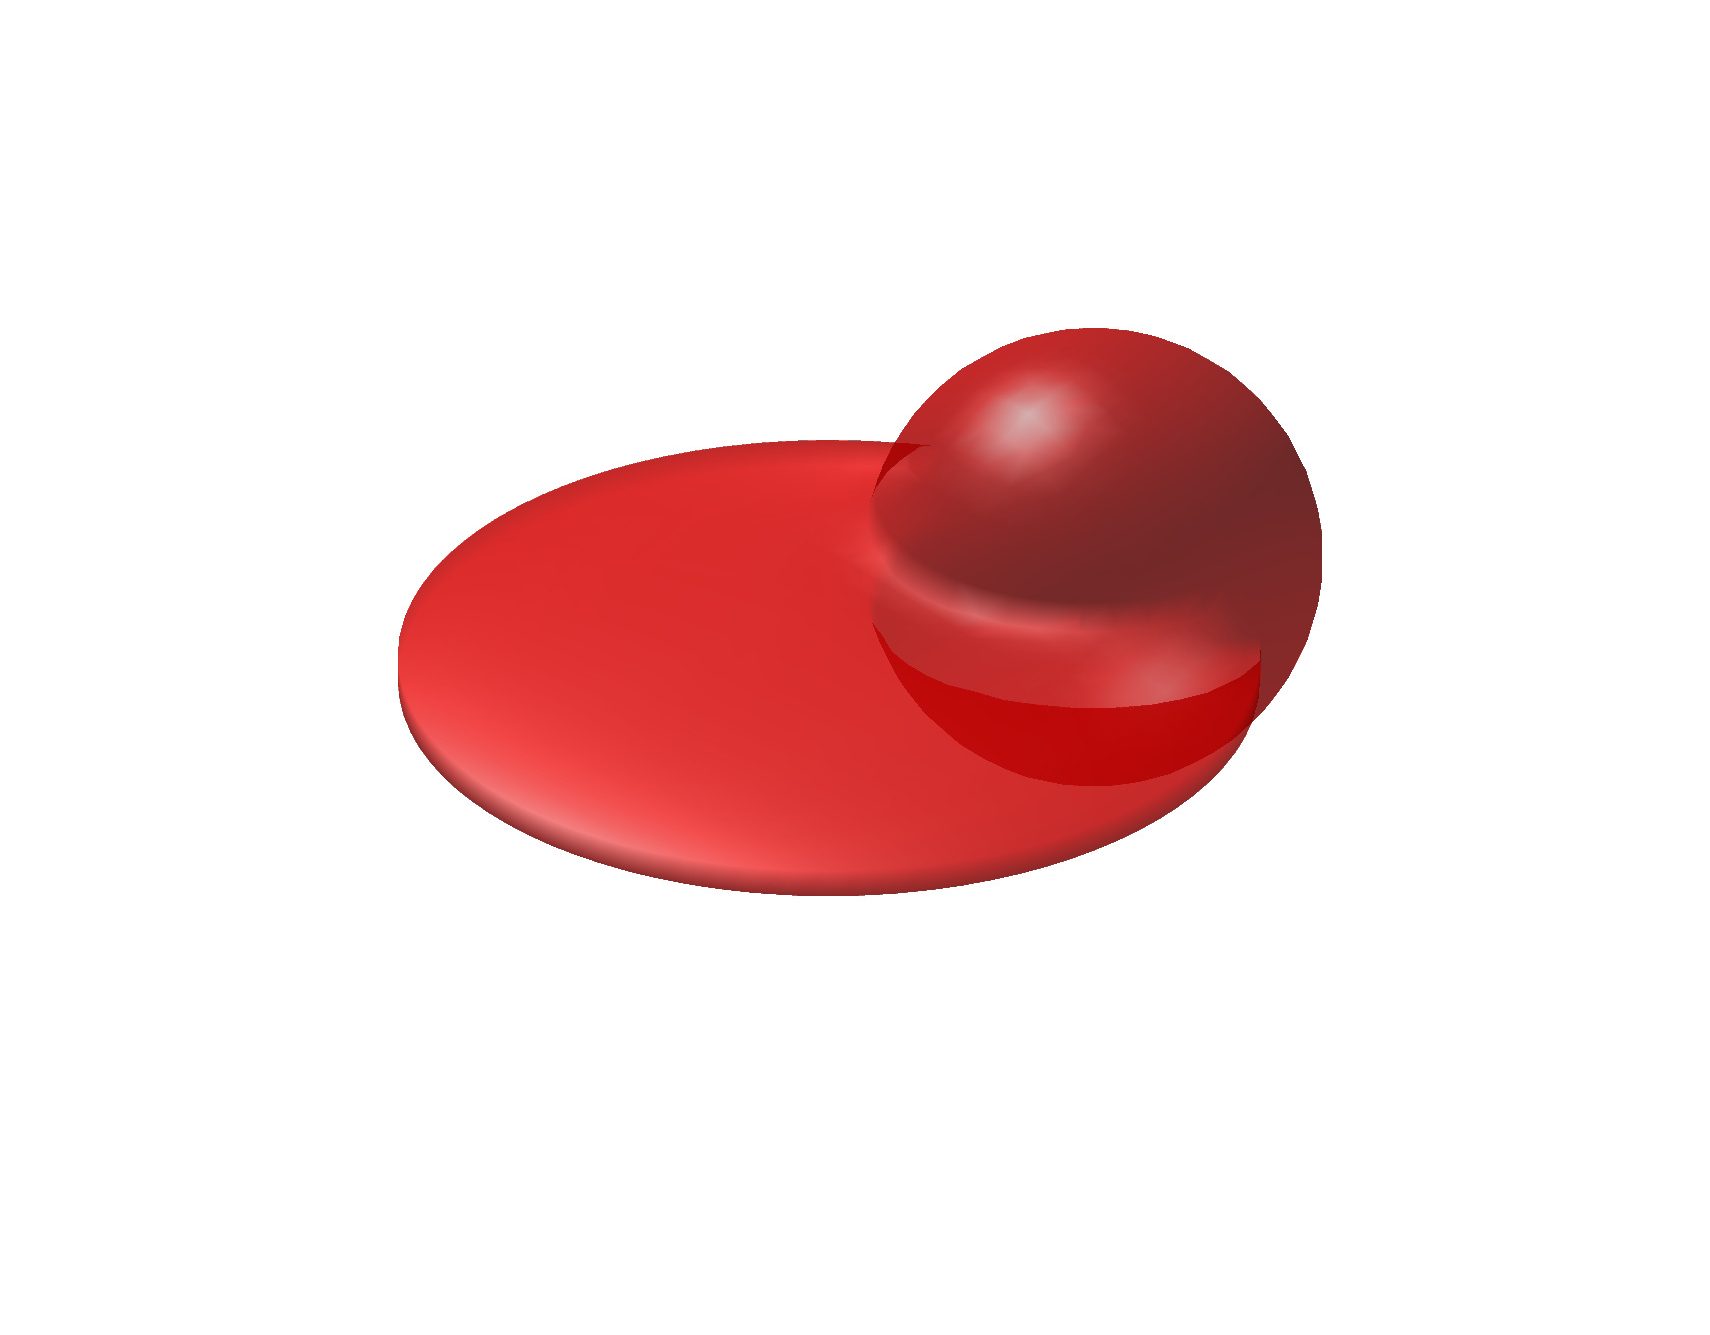
\includegraphics[width=.32\textwidth]{./figs/union.pdf} & 
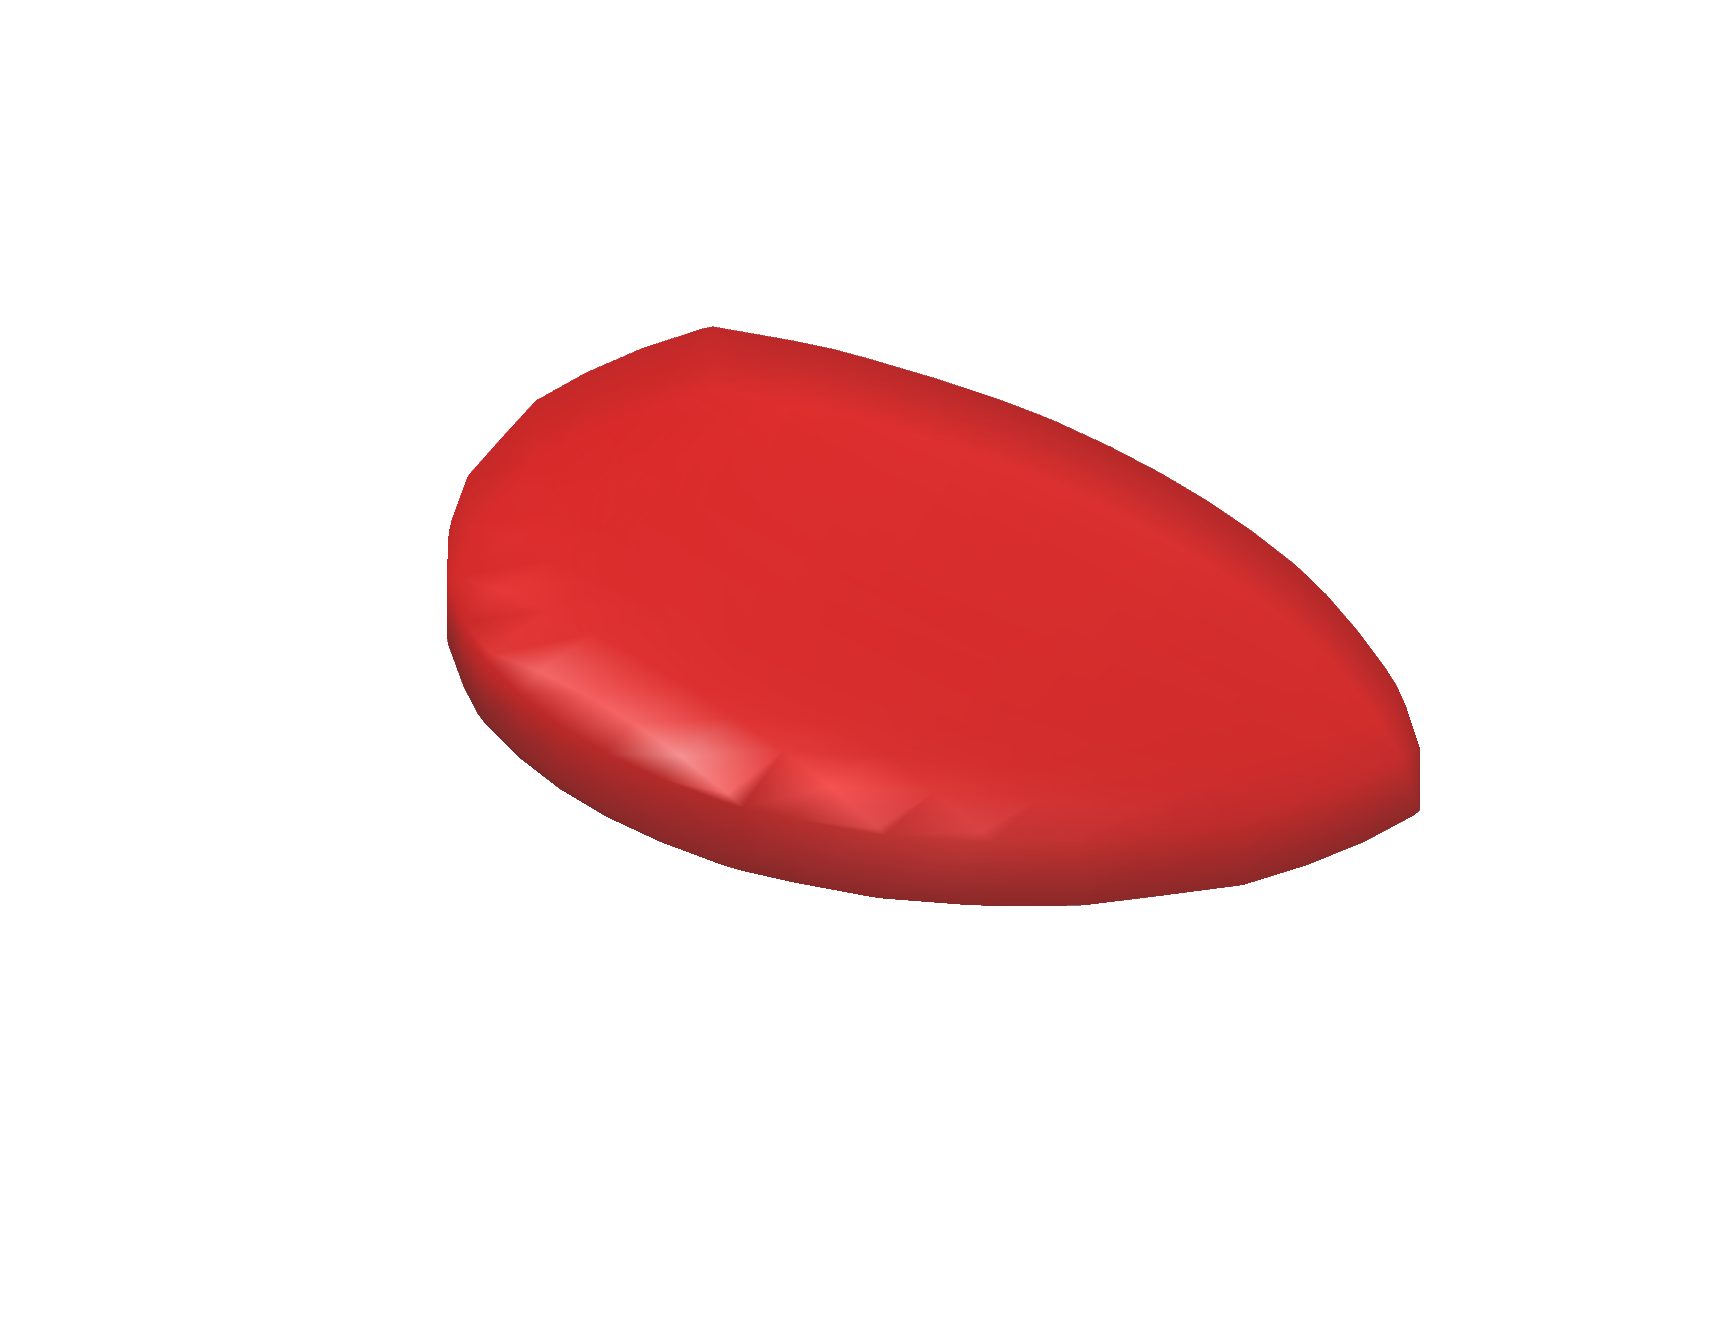
\includegraphics[width=.32\textwidth]{./figs/intersect.pdf} & 
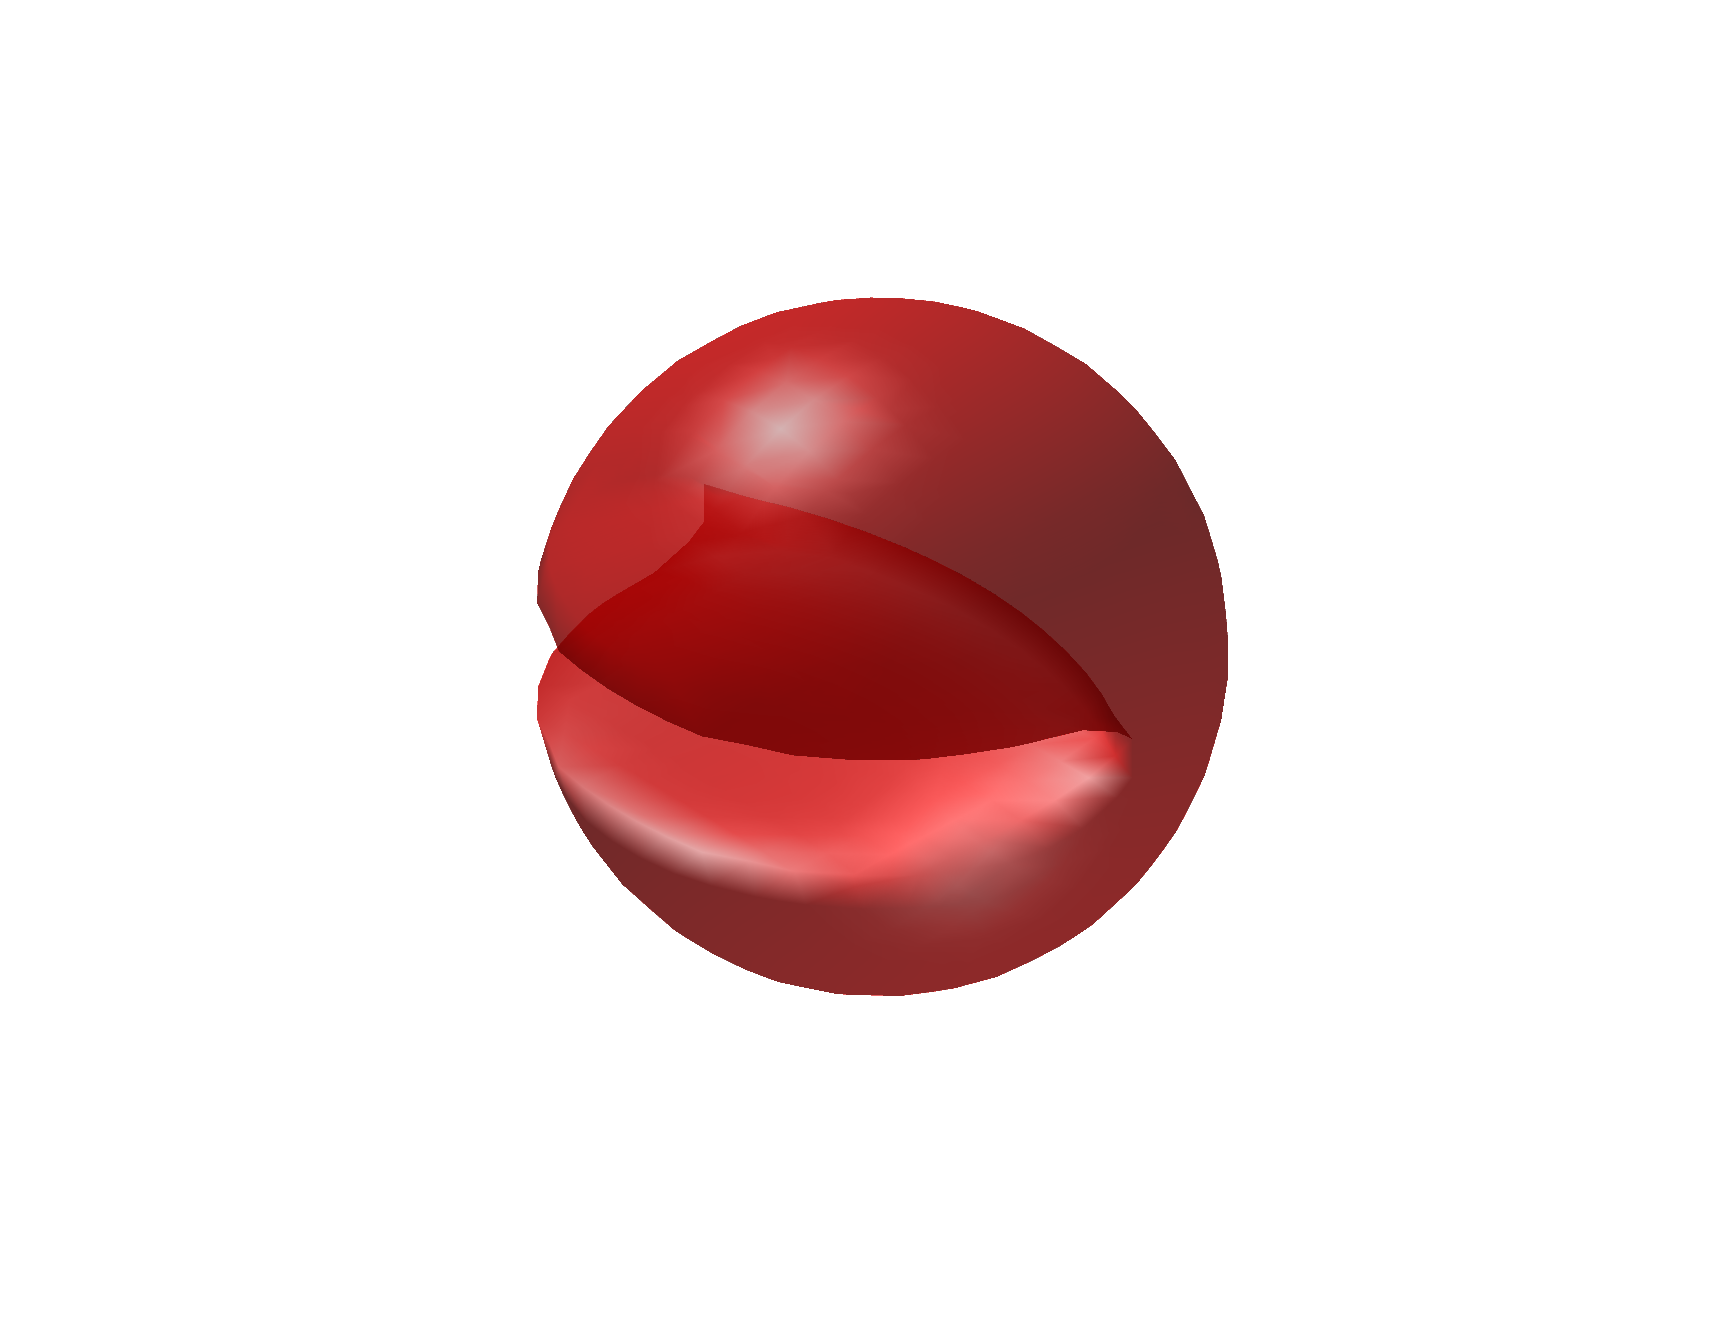
\includegraphics[width=.32\textwidth]{./figs/diff.pdf}\\
$f \cup g$ & $f \cap g$ & $f \setminus g$ 
\end{tabular}
\end{frame} 

\begin{frame}[fragile]
\frametitle{Optical cross section (OCS)}
\begin{itemize}
\item Accumulate reflectance over a target surface
\item Discrete: Sum over triangular facets 
\item Continuous: Analytic formulas (use R-functions); 
used \verb+chebfun+ for computing integrals
\end{itemize}
\centerline{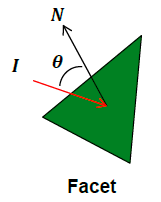
\includegraphics[scale = 0.5]{./figs/facet.png} \: 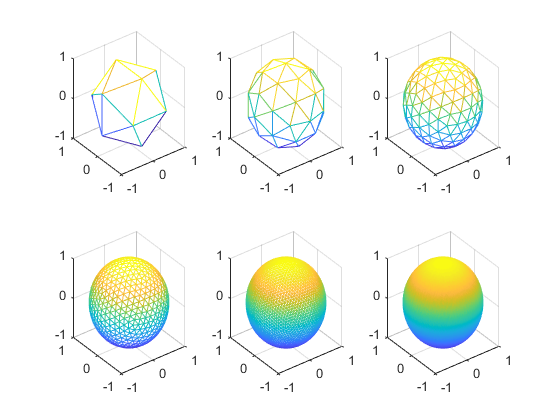
\includegraphics[scale = 0.5]{./figs/icosahedron.png}}
\end{frame}

\begin{frame}[t]
\frametitle{The Blinn--Phong model}
\centerline{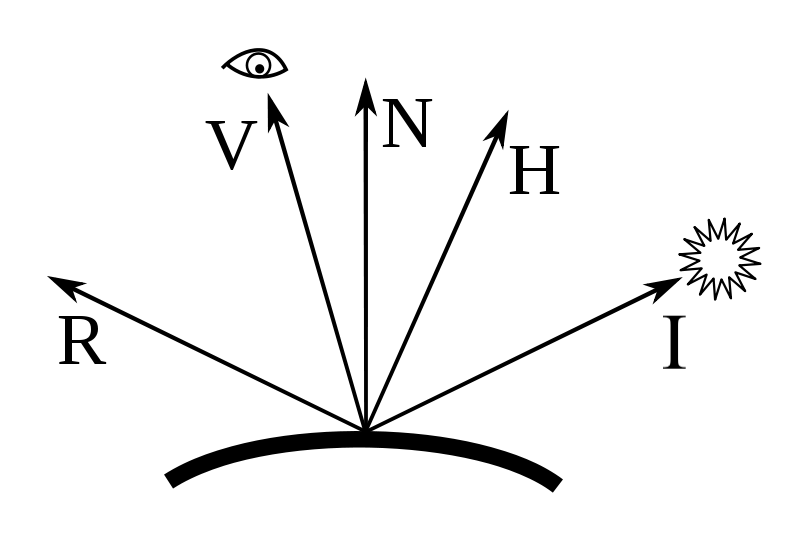
\includegraphics[scale=0.22]{./figs/ModelVectors}}
$$\text{BRDF}(\mathbf{I},\mathbf{V}) = \big(<\mathbf{H},\mathbf{N}>\big)^\alpha \text{ for } \alpha \geq 0$$
\centerline{where the \textit{halfway vector} $\mathbf{H}$ is defined as $(\mathbf{I} + \mathbf{V})/\|\mathbf{I} + \mathbf{V}\|$}
\begin{itemize}
\item Modification of Phong model
\item BRDF: \textit{Bistatic reflectance distribution function}
\end{itemize}
\end{frame}

\begin{frame}[t]
\frametitle{Blinn--Phong as MRDF}
\begin{itemize}
\item MRDF: \textit{Monostatic reflectance distribution function}
\item Case where $\mathbf{I} = \mathbf{V}$
\end{itemize}
\centerline{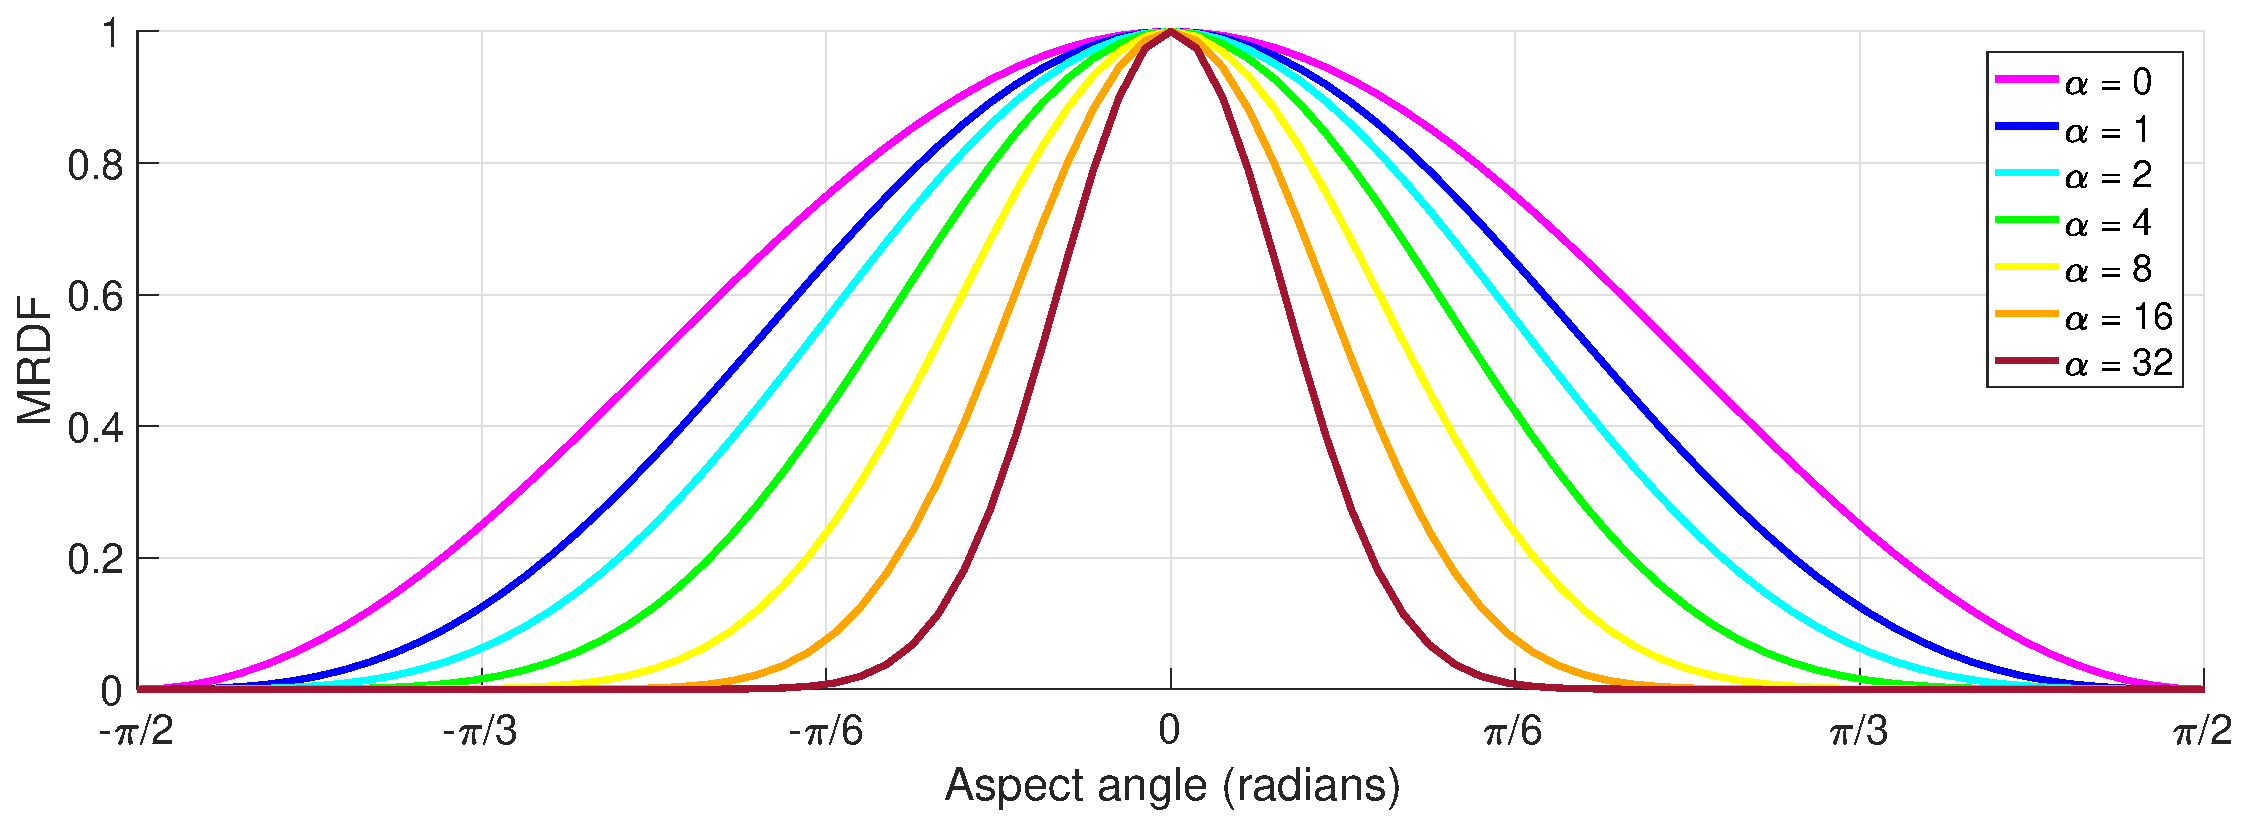
\includegraphics[scale=0.3]{./figs/MRDFs}}
\end{frame}

\begin{frame}
\frametitle{Blinn--Phong as BRDF}
\centerline{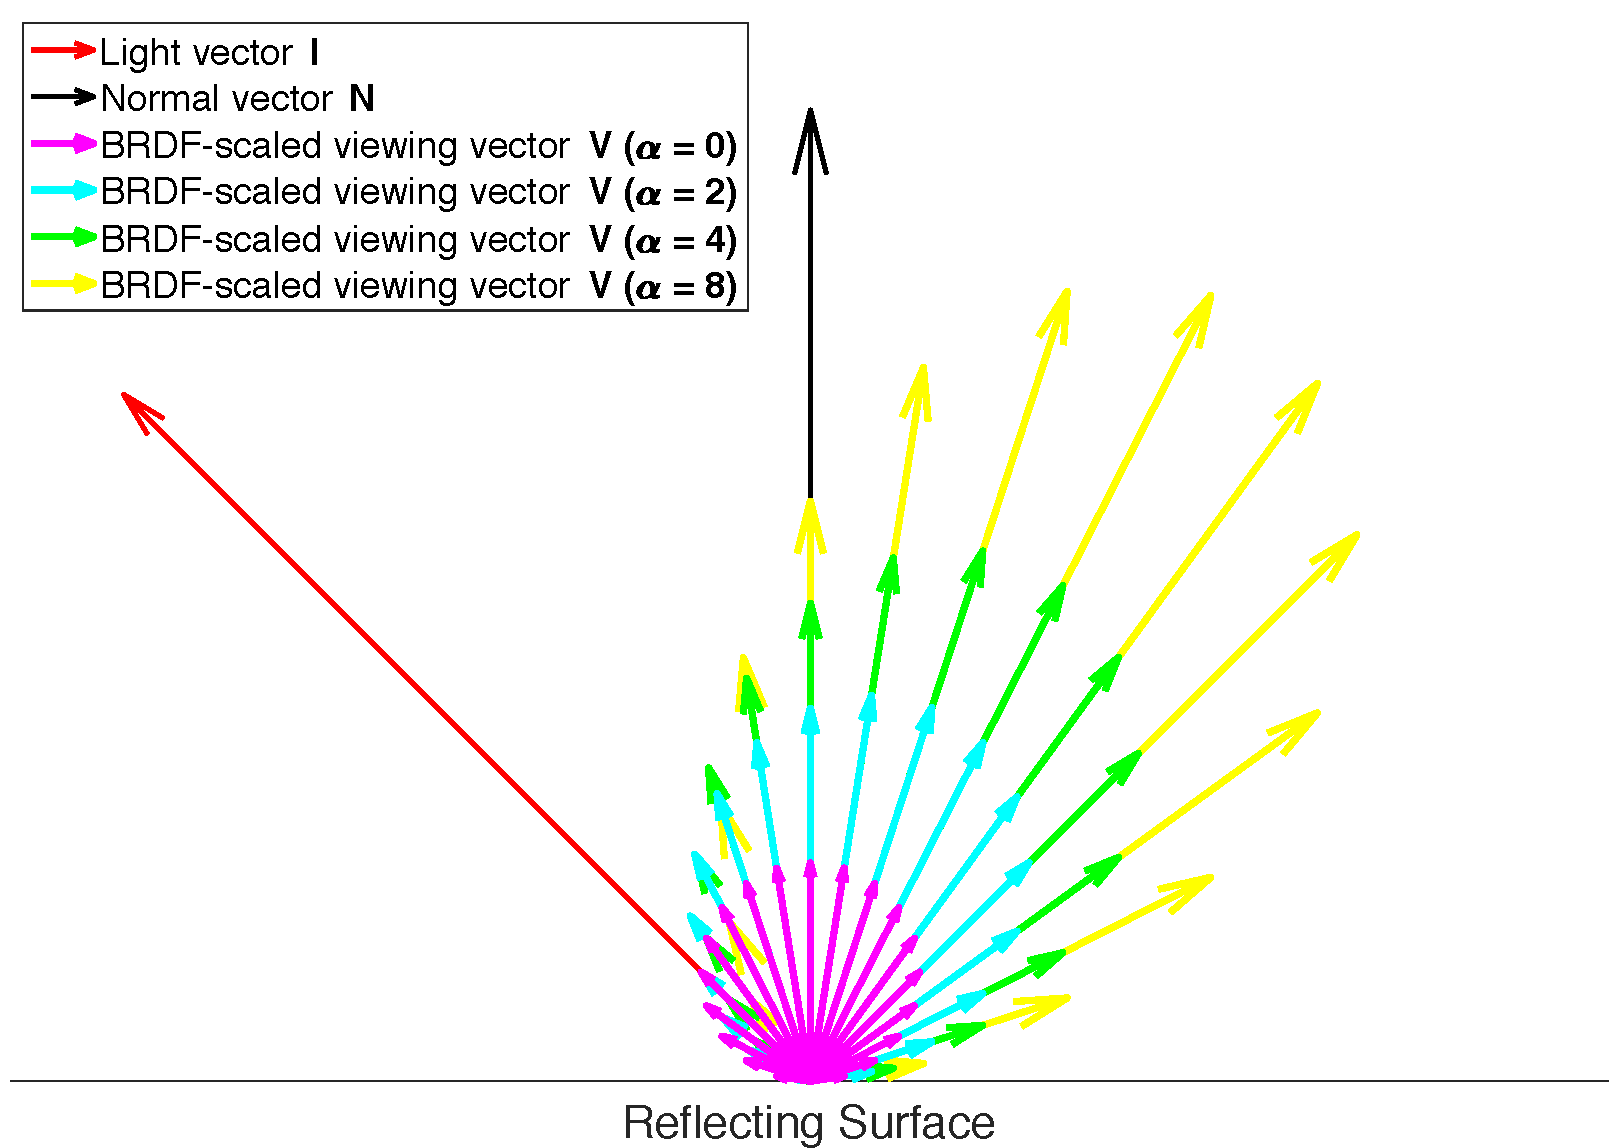
\includegraphics[scale=0.4]{./figs/BRDF_Vectors.pdf}}
\end{frame}

\begin{frame}[t]
\frametitle{Analytic benchmark: the sphere}
\begin{itemize}
\item Unit sphere (spherical coordinate)
\item Light source: fixed at the direction $(\theta,\phi) = (\frac{\pi}{2},\frac{\pi}{2})$
\item Detector: orbiting on $xy$-plane
\item Varying specular highlight
\end{itemize}
\begin{multicols}{2}
\centering 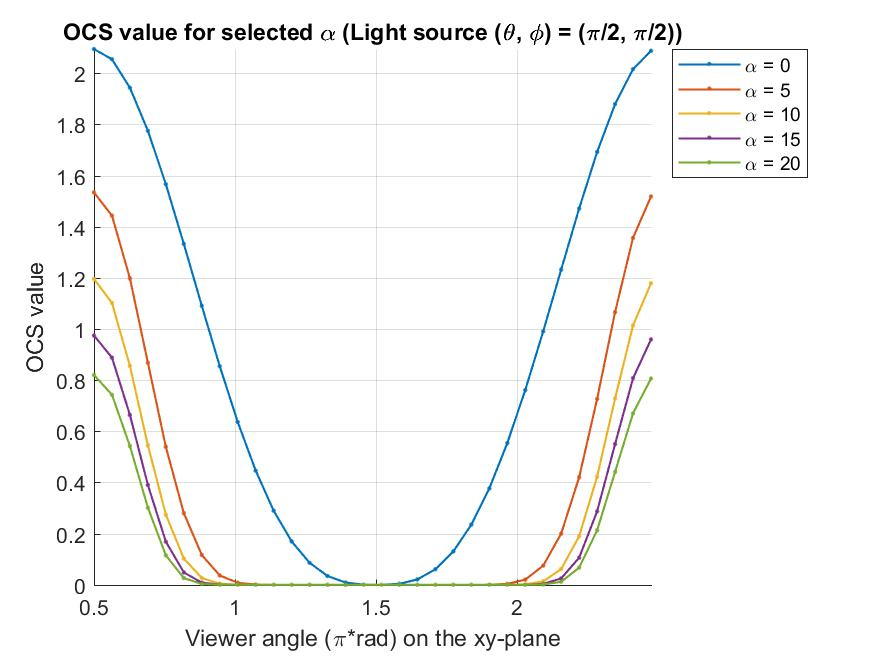
\includegraphics[scale=0.13]{./figs/OCS_parallel_plane}
\begin{figure}
\centering 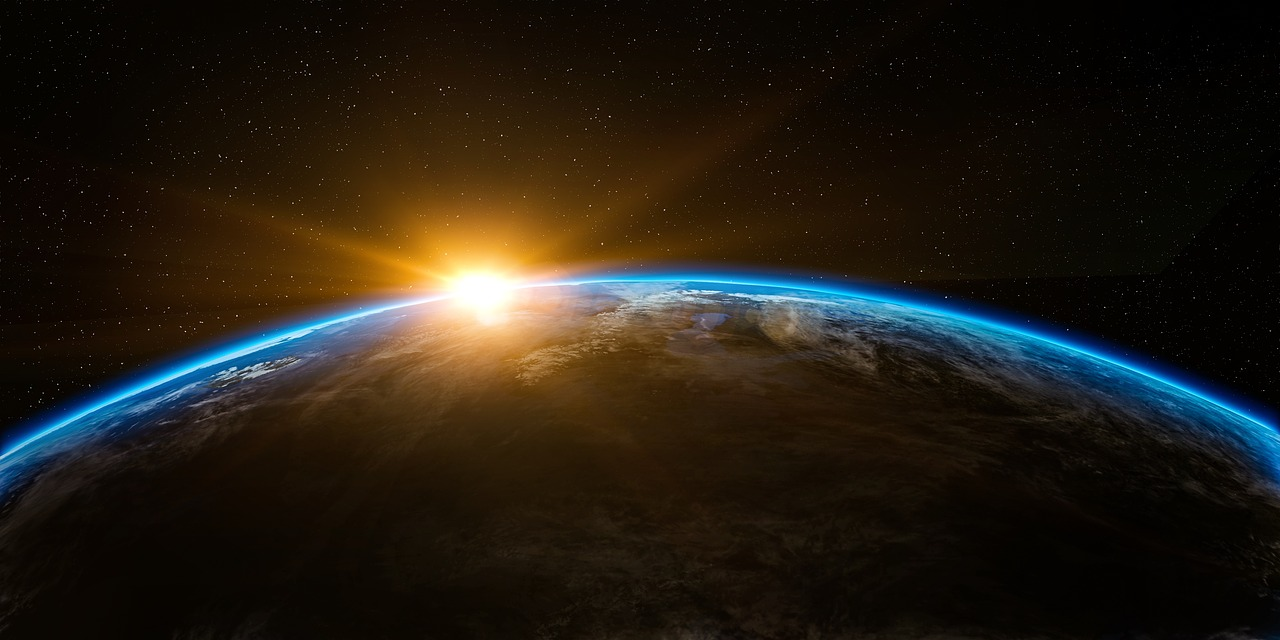
\includegraphics[scale=0.1]{./figs/orbiting_example}\caption{qimono.
 pixabay. 2016}
\end{figure}
\end{multicols}
\end{frame}

\begin{frame}[t]
\frametitle{Chebfun and the sphere (cont'd)}
\begin{itemize}
\item Unit sphere
\item Light source: fixed at the direction $(\theta,\phi) = (0,0)$
\item Detector: orbiting on $xy$-plane
\item Varying specular highlight
\end{itemize}

\centering 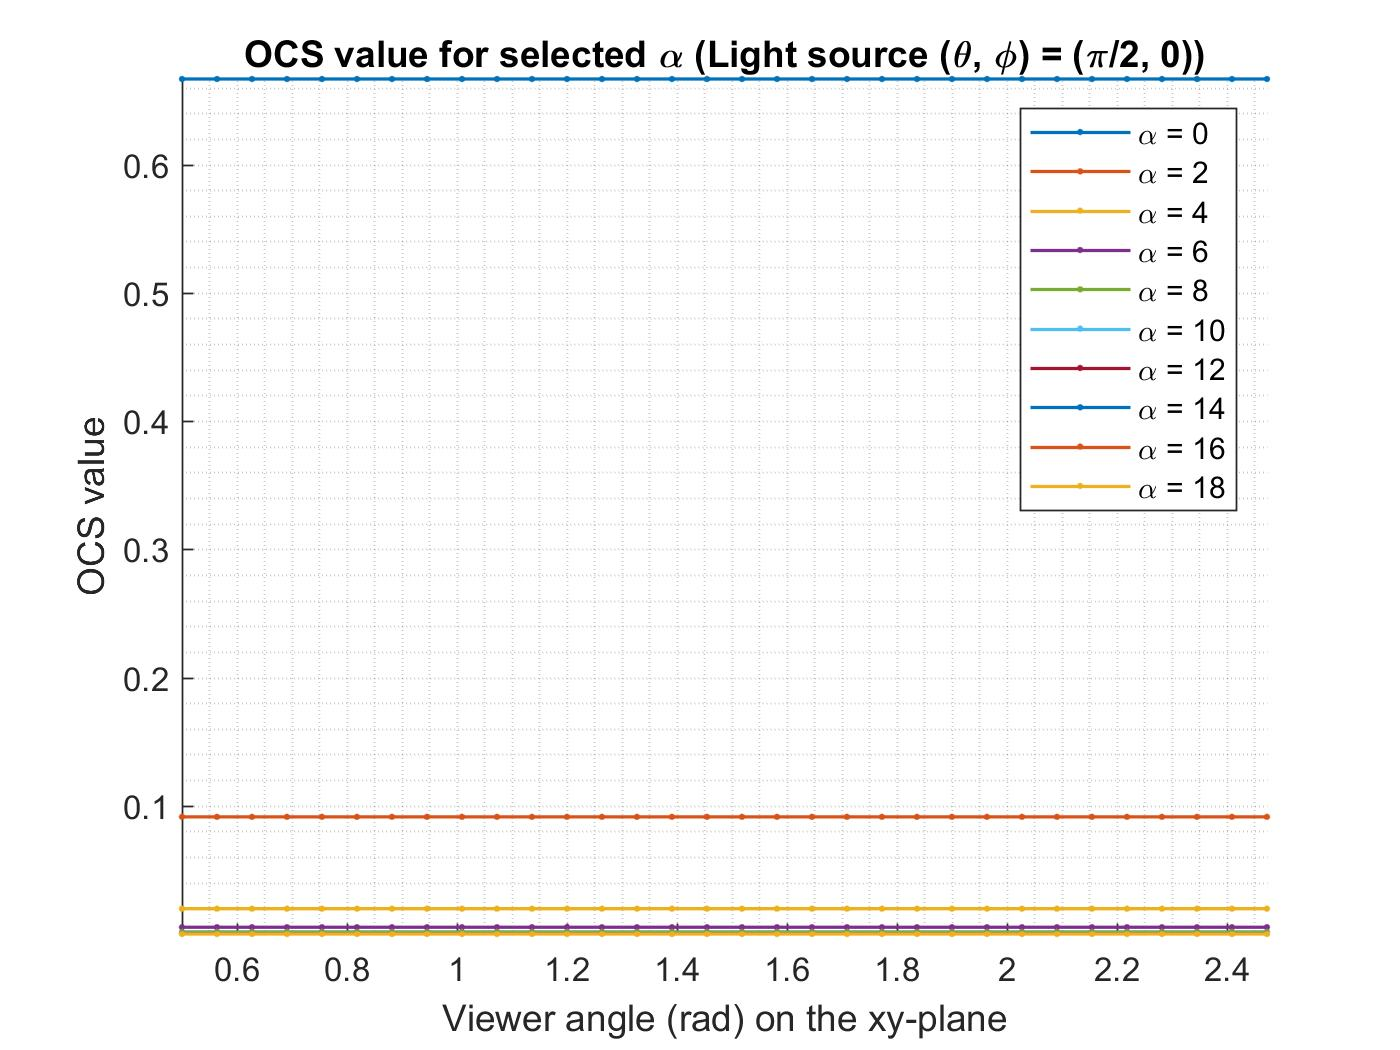
\includegraphics[scale=0.13]{./figs/OCS_perpendicular_plane}
\end{frame}


\begin{frame}[t]
\frametitle{Multipath}
\end{frame}


\begin{frame}[t]
\frametitle{Conclusion and future work}
\begin{itemize}
\item Implicit representations of composite objects readily obtained from R-functions 
\item Advantages of continuous OCS computation over facet method for simple shapes
\item 
\item Investigation of continuous solutions for more complex/``sharper" objects 
\end{itemize}
\end{frame}

\end{document}


%% Image references: 
 
% Satellite.jpg: https://www.newscientist.com/article/2113311-first-ever-lightning-mapping-satellite-set-for-take-off/ 
 
% ModelVectors.jpg: By Martin Kraus - Own work, CC0, https://commons.wikimedia.org/w/index.php?curid=15534756
